\section{Experiments}
\label{sec-quant}
\begin{figure}
  \centering
  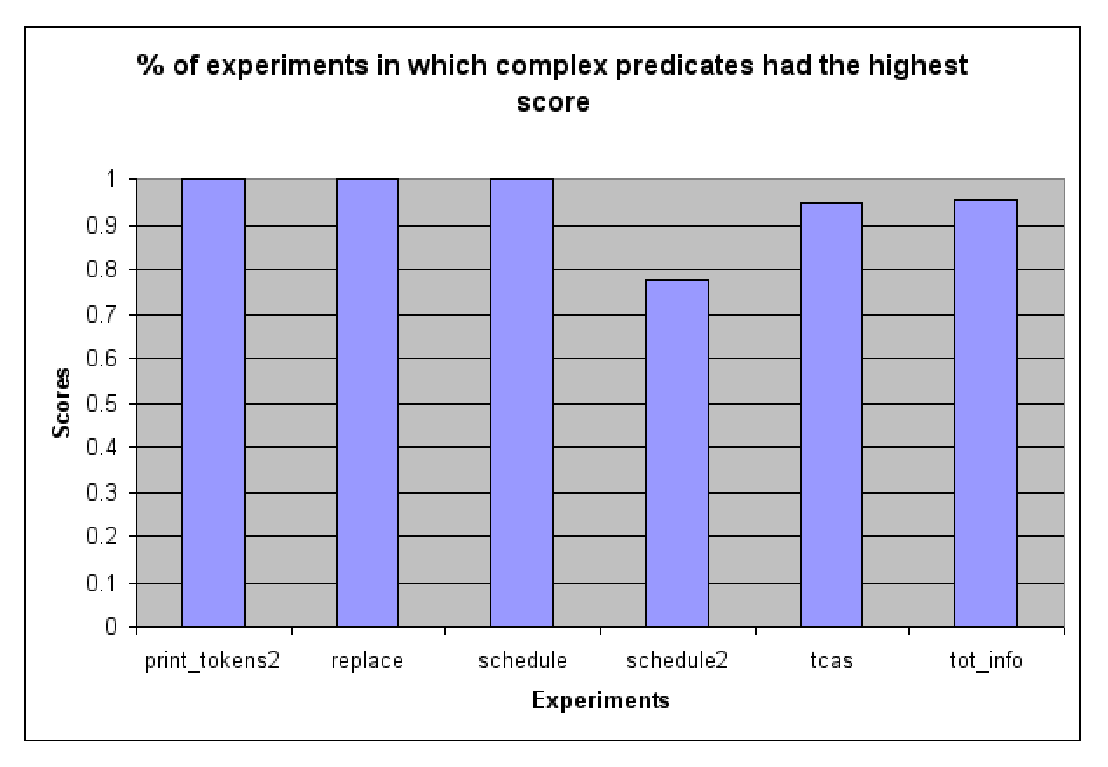
\includegraphics[width=\columnwidth]{charts/top-pred}
  \label{fig-top-pred}
  \caption{Complex predicates having the highest score}
\end{figure}

\begin{figure}
  \centering
  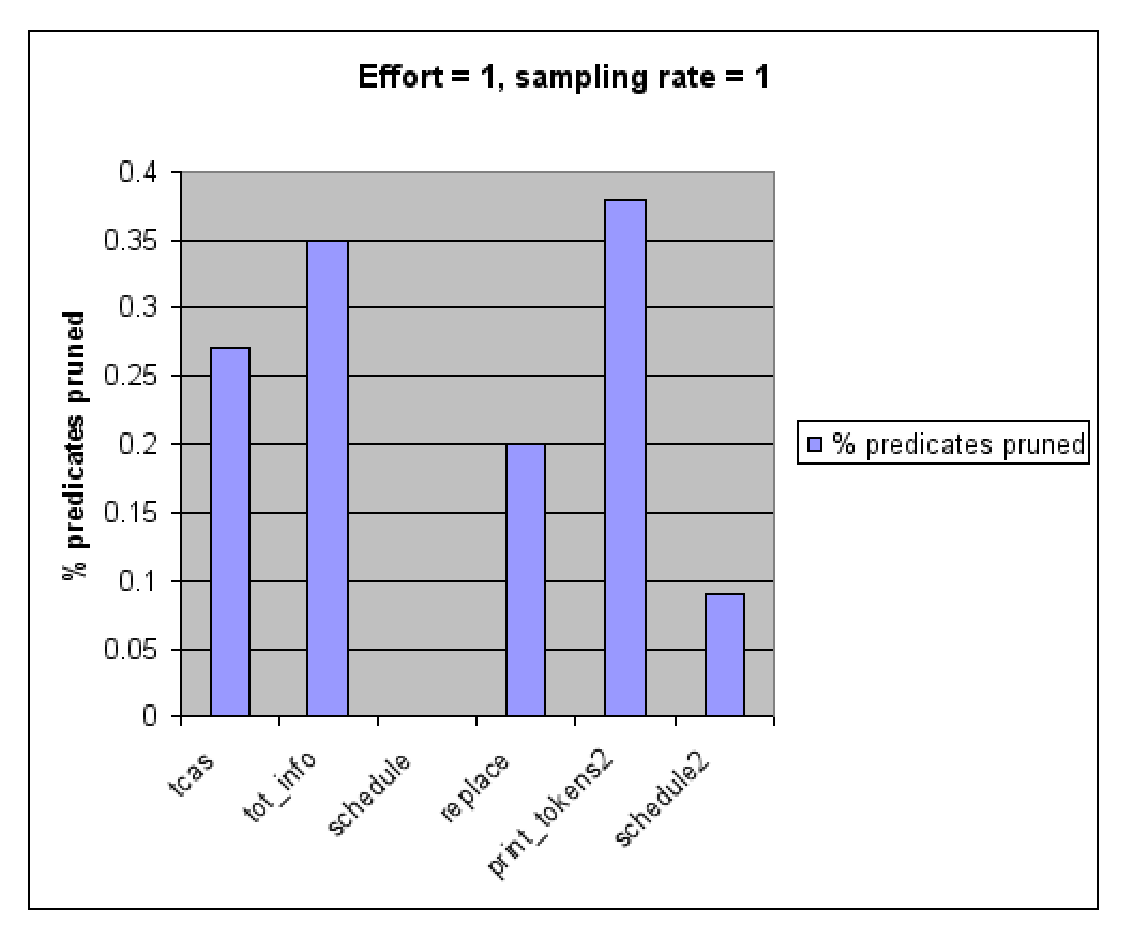
\includegraphics[width=\columnwidth]{charts/pruning}
  \caption{Improvement from pruning}
  \label{fig-pruning}
\end{figure}

\begin{figure}
  \centering
  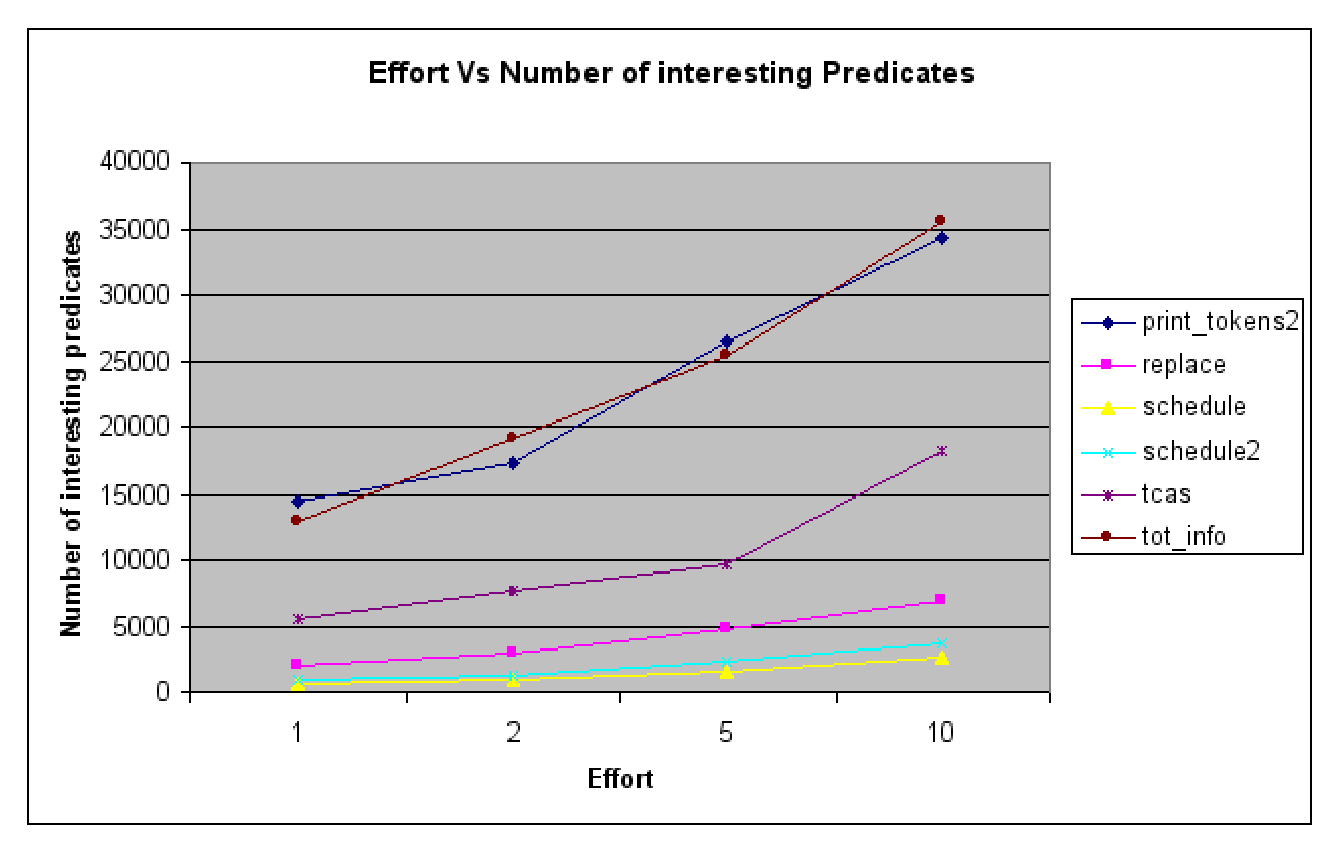
\includegraphics[width=\columnwidth]{charts/effort}
  \caption{Variation of number of interesting predicates with $effort$}
  \label{fig-effort}
\end{figure}

This section presents quantitative data about the ideas presented in previous sections.  This data was collected using the Siemens test suite~\cite{257766}.  There are two configurable parameters for the experiments: the rate of sampling and $effort$ (described in ~\autoref{sec-metrics}).  Unless specified, the default sampling rate is 1 (i.e. complete data collection) and the default $effort$ is 5\% (only predicates that are reachable from each other by exploring less than 5\% of the program are considered).

\subsection{Top Scoring Predicates}
~\autoref{fig-top-pred} plots the percentage of variants within each program for which a complex predicate had the highest score among all predicates.  The value is 100\% for \texttt{print\_tokens2, replace} and \texttt{schedule} and is close to 100\% for the other programs.  The results shown in ~\autoref{fig-top-pred} combined with the case studies in ~\autoref{sec-qual} demonstrates the usefulness of complex predicates.

\subsection{Improvement from Pruning}
~\autoref{fig-pruning} shows the percentage of complex predicates that are pruned by the optimizations discussed in ~\autoref{sec-pruning} and the metrics in ~\autoref{sec-metrics}.  For each program, the y-axis shows the contribution of the two kinds of pruning.  On average, the usefulness metrics prune 54\% of complex predicates and the optimizations in ~\autoref{sec-pruning} prune 15\% of complex predicates.  Only 31\% of the complex predicates are actually computed.

\subsection{Effect of the $Effort$ Parameter}
~\autoref{fig-effort} has one curve for each program showing how the number of interesting predicates (~\autoref{dfn3}) varies at four different values - 1, 2, 5, 10 for $effort$.  As expected, the higher the $effort$, more predicates are evaluated and so more interesting predicates are found.  This experiment serves as a sanity check for the implementation.

\subsection{Effect of Sampling Rate}
\label{sec-sampling}
Include the graphs